\chapter{Background}

In this chapter, we describe the concept of data provenance. 

%\section{Cyber-Physical Systems}
%CPS is the combination of computation and physical component 


%\section{Internet of Things (IoT)}
%There is no standard definition for IoT, however, researchers have tried to define the concept of connected ``things". The concept of IoT was proposed by Mark Weiser in the early 1990s \cite{Mattern} which represents a way in which the physical objects, ``things", can be connected to the digital world. Gubbi et al \cite{park_provenance-based_2012} defines the IoT as  an interconnection of sensing and actuating devices that allows data sharing across platforms through a centralized framework. We define (IoT) as follows:
%
%\begin{definition}
%The Internet of Things (IoT) is a network of heterogeneous devices with sensing and actuating capabilities communicating over the internet. 
%
%\end{definition}
%
%The notion of IoT has been attributed to smart devices. The interconnectivity between various heterogeneous devices allows for devices to share information in a unique manner. Analytics is a driving force for IoT. With analytics, devices can learn from user data to make smarter decisions. This notion of smart devices is seen in various commercial applications such as smartwatches, thermostats that automatically learns a user patterns. The ubiquitous nature of these devices make them ideal choices to be included in consumer products. IoT architecture consists of four distinct layers: The sensor and actuator layer, device layer, gateway layer and the cloud layer. 
%
%\par With the recent data explosion \cite{emc_bigdata} due to the large influx in amounts of interconnected devices, information is disseminated at a fast rate and with this increase involves security and privacy concerns. Creating a provenance-aware system is beneficial to IoT because it ensures the trust and  integrity of interconnected devices. Enabling provenance collection in IoT devices allows these devices to capture valuable information which enables backtracking in an event of a malicious attack. We take a holistic approach to provenance collection by looking at how provenance information is collected across an IoT architectural framework.

 
%  \subsection{IoT Architecture}
%
%IoT architecture represents a functional hierarchy of how information is disseminated across multiple hierarchies contained in an IoT framework; from devices which contain sensing and actuating capabilities to massive data centers (cloud storage). Knowing how information is transmitted across layers allows a better understanding on how to model the flow of information across actors contained in an IoT hierarchy. 
%\par Figure \ref{iot_architecture} displays the IoT architecture and the interactions between the respective  layers. The base of the architectural stack consist of sensors and actuators which gathers provenance information and interacts with the device layer. The device layer consists of devices (e.g mobile phones, laptops, smart devices) which are responsible for aggregating data collected from sensors and actuators. These devices in turn forwards the aggregated data to the gateway layer. The gateway layer routes and forwards data collected from the device later. It could also serve as a medium of temporary storage and data processing. The cloud layer is involved with the storage and processing of data collected from the gateway layer. Note that the resource constraints decreases up the architectural stack with the cloud layer having the most resources (memory, power computation) and the sensor-actuator layer having the least. 
%
%
%\begin{figure}[h]
%\begin{center}
%
%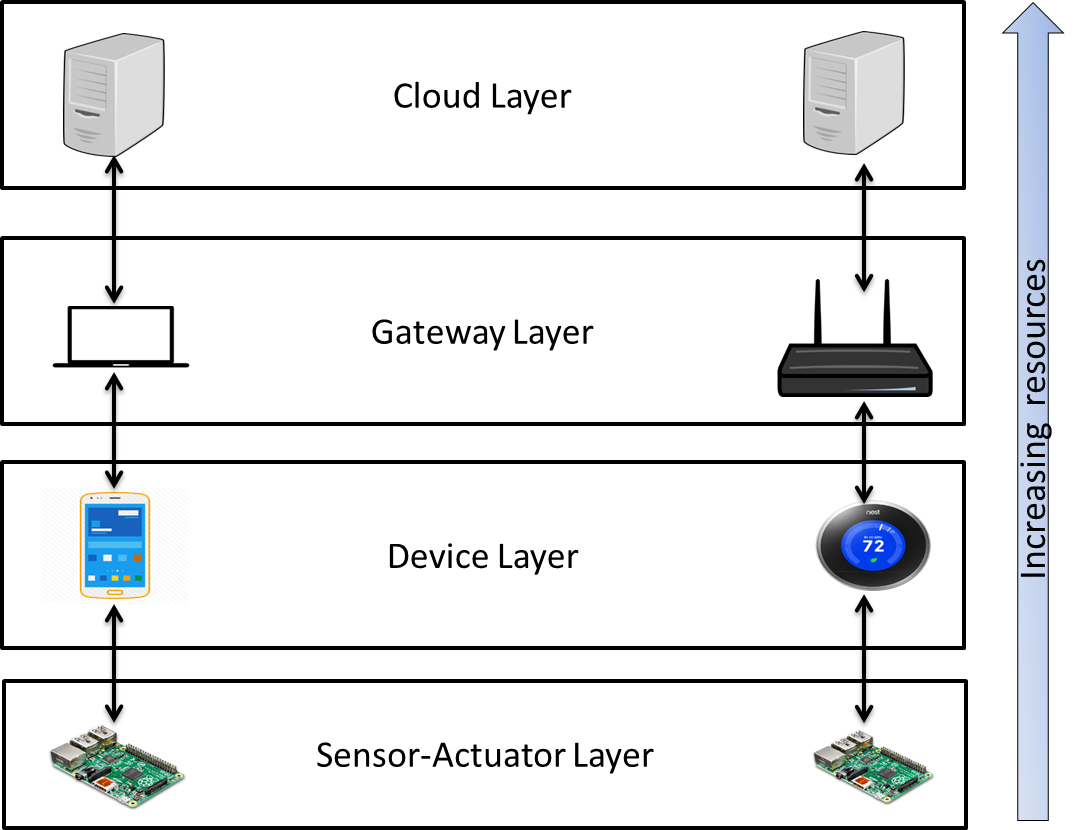
\includegraphics[height=3.0in]{iot_architecture.png}
%\end{center}
%\caption{IoT Architecture Diagram. The arrows illustrates the interaction between data at various layers on the architecture.}
%\label{iot_architecture}
%
%\end{figure}
%
%\section{Cyber- Physical System}


%\subsection{Anomaly Detection}
%
%The notion of what constitutes an anomaly is often domain specific. Hawkins defines an anomaly as an ``observation which deviates so much from the other observations as to arouse that it was generated by a different mechanism" \cite{hawkins}. In computing, an anomaly often indicates the presence of a malicious intrusion or a system fault. For example, an anomaly could be a sudden increase in web traffic of a web server which could be indicative of a denial of service attack. Additionally, in a critical care health device such as a pacemaker, an anomalous event could be detrimental to the health of a patient which could result in the loss of life. 
%
%%Anomaly detection consists of two phase, learning phase also known as the training phase and the test also known as the detection phase. In the training phase, the system collects training dataset. This data is considered to be a representation of the system's normal daily activity and free from malicious events. Once training dataset has been collected, the system's activities are further observed. This part is known as the testing phase. In the testing phase,  observed system behavior is compared to the learning phase to determine is an anomaly exists between the two. A threshold as defined by domain experts is used to determine if the observed data is considered an anomaly.
%
%%Data labels are grouped into three major categories. Supervised anomaly detection, semi-supervised anomaly detection, and unsupervised anomaly detection. In supervised anomaly detection approach, training data contains instances of normal and anomalous data. Incoming data is classified based on the training data category. In semi-supervised approach, only one class of training data is collected, normal data. Incoming data that does not fit the normal class as specified by a threshold is regarded as an anomalous. In the training phase, most anomaly detection techniques use data derived from the normal system behavior.  This is referred to as one class classification. In unsupervised approach, there are no training dataset. it is believed that normal data is clustered around each and occurs more frequently than an anomaly. This is a widely used form of anomaly detection since training data which is hard to get is not requited. 
%
%
%Anomaly detection involves the use of rule-based, statistical, clustering or classification techniques to determine normal or anomalous data instances. The process of determining all anomalous instances in a given dataset or system is a complex task. A major challenge in anomaly detection is providing the right feature set from the data to use for detection. Another challenge exists in defining what constitutes as normal system behavior. Most anomaly detection using point based data often fail to include the dependencies that exist between data points.   

\section{Data Provenance}

Provenance is defined as ``The place of origin or earliest known history of something"~\cite{TCDP1999}. However, provenance and lineage are used interchangeably to denote the origin of something and transformation(s) that occurred to it over time. The notion of provenance originates from the art world, where an art piece auctioned is accompanied by a paper trail that denotes the artwork's chain of custody. This trail allows a buyer to ascertain the authenticity of the artwork. Likewise in computing, provenance provides a holistic history of data transformations that occur on a data object from inception to its present state. 

Data provenance can ensure data integrity \cite{Bertino2015} and establish causality between data objects through information-flow tracking.
Characteristic information provided by provenance include the who, where, when, and what of data transformation. \textbf{Who} identifies an actor responsible for a particular transformation of a data object. An example of ``who" in a CPS use case is a sensor, which is identified as the ultimate progenitor of values derived from its sensor readings. \textbf{Where} provides the location of a transformation, for example a geolocation for the sensor. \textbf{When} associates time with a transformation, e.g., a timestamp obtained when a particular sensor reading was taken. \textbf{What} denotes the kind of transformation, such as a {\em read} operation or a {\em send} operation.

Provenance has been applied to database management to track the derivation of a query, in forensic analysis to determine what activities led to a system event~\cite{Bates2014LetSB, Lu:2010:SPE:1755688.1755723, 6542529}, in scientific experimentation for experiment reproducibility~\cite{chimera, Davidson:2008:PSW:1376616.1376772, altintas, Oinn2004TavernaAT}, and in intrusion detection~\cite{Xie_yulani, Fadolalkarim, 203308} to detect what activity might be responsible for a malicious compromise.

The increase in applications of provenance has led to provenance collection systems to support them. For example, within the context of the operating system, PASS~\cite{muniswamy_reddy} and HiFi~\cite{hi_fi} are two Linux-based provenance collection systems developed to capture interactions between files and system call events. In the scientific community, Chimera~\cite{chimera} and myGrid~\cite{Oinn2004TavernaAT} collect provenance to support scientific experiment workflow reproducibility. Notably, most of these applications are tailored for large-scale, memory-intensive applications that are difficult to adapt directly to memory-constrained CPS devices.





%The Oxford English dictionary defines provenance \cite{TCDP1999} as ``the place of origin or earliest known history of something". An example of provenance can be seen with a college transcript. A transcript is the provenance of a college degree because it outlines all of the courses satisfied in order to attain the degree.
%
%
%In the field of computing, data provenance, also known as  data lineage, can be defined as the history of all activities performed on entities from its creation to its current state. Cheney et al. \cite{cheney_provenance_2009} decribes provenance as the origin and history of data from its lifecycle. Buneman et al \cite{buneman_why_2001} describes provenance from a database perspective as the origin of data and the steps in which it is derived in the database system.  Provenance involves two granularity levels: fine-grained provenance and coarse-grained provenance. Fine-grained provenance \cite{glavic_case_2011} entails the collection of a detailed level of provenance. Coarse grained provenance, on the other hand, is a collection of a summarized version of provenance. Data provenance has immense applications and has been explored in the areas of scientific computing \cite{groth, altintas} to track how an experiments are produced, in business to determine the work-flow of  a process, and in computer security for forensic analysis and intrusion detection \cite{bates_towards_2013, muniswamy_reddy_provenance_2010, muniswamy_reddy} . 
%
%
%Provenance denotes the who, where and why of data \cite{cheney_provenance_2009}. An example of provenance for a software system is a web server's log file. This file contains metadata for various request and response time and the ip address of all host systems that requests information from the server. This log file identifies the data object (i.e. Web server), transformations that occurs on this object (e.g read write connections) and the state of the data object. Provenance data is represented as an acyclic graph which denotes casual relationship and dependencies between entities. 
%
%\par Provenance ensures trust and integrity of data \cite{Bertino2015}. It outlines causality and dependency between all objects involved in the system and allows for the verification of the source of data. Causality and dependency are used to determine the relationship between multiple objects. The relationship in which provenance denotes can in turn be used in digital forensics \cite{zawoadfecloud} to investigate the cause of a malicious attack and also in intrusion detection systems to further enhance the security of computing devices. 
% 
%
%Characteristic information provided by provenance include the who, where, when, and what of data transformation. \textbf{Who} identifies an actor responsible for a particular transformation of a data object. An example of ``who" in a CPS use case is a sensor, which is identified as the ultimate progenitor of values dervied from its sensor readings. \textbf{Where} provides the location of a transformation, for example a geolocation for the sensor. \textbf{When} associates time with a transformation, e.g., a timestamp obtained when a particular sensor reading was taken. \textbf{What} denotes the kind of transformation, such as a {\em read} operation or a {\em send} operation.

%\section{Comparing Provenance with Log Data and Metadata}
%
%Provenance data, log data and metadata are key data concepts that often are used interchangeably. We try to address the differences and similarities between provenance data, metadata and log data.
%
%\subsection{Provenance and Metadata}
%Metadata and provenance are often considered related but yet subtle distinctions exist. Metadata contains descriptive information about data. Metadata can be considered as provenance when there exists a relationship between objects and they explain the transformation that occurs. In summary,  metadata and provenance are not the same, however an overlap exists. Metadata contains valuable  provenance information but not all metadata is provenance information. 
%
%
%\subsection{Provenance and Log data}
%Log data contains information about the activities of an operating system or processes. Log data can be used as provenance because It contains data trace specific to an application domain. Log files might contain unrelated information such as error messages, warnings which might not be considered as provenance data. Provenance allows for specified collection of information that relates to the change of the internal state of an object. In summary, log data could provide insight to what provenance data to collect. 


 

%
%\section{IoT Application Use Case}

\section{Model for representing data provenance}

%In order to represent the right kind of provenance information, we need to satisfy the who, where, how, and what of data transformations. Provenance data can be represented using a provenance model in a modeling language such as, PROV\-DM which is represented in serialized form as a JSON object. This model displays the causal relationship of data objects. We propose a model that contains information such as sensor readings, device name, and device information. Details on the PROV-DM and PROV-JSON are outlined below.


To facilitate the creation of cross-platform provenance, an abstract representation of provenance typically uses a directed acyclic graph (DAG) in which vertices correspond to data and edges to interactions between data. A selection of vertex types and edge relationships constitutes a provenance model. The W3C standardizes a provenance ontology and a provenance data model, PROV-DM, to enable interchangeable provenance across heterogeneous systems. We adopt notions from the PROV-DM in the creation of Prov-CPS.


%We adopt the Provenance Data Model (PROV-DM) \cite{prov_dm}, a W3C standard which conforms to Provenance Ontology (PROV-O) and is used to depict dependencies between entities, activities and agents (digital or physical). PROV-DM creates a common model that allows for interchange of provenance information between heterogeneous devices and is represented serialized in three formats:  XML, JSON and RDF. 

\par PROV-DM contains two major components: types and relations.  Types can be entities, activities, or agents. An entity is a physical or digital object. An activity represents some form of action that occurs over time.  An agent takes ownership of an entity, or performs an activity. Figure \ref{prov_rep} illustrates the types and relations contained in PROV-DM and their graphical representation. Entities, activities and agents are represented as oval, rectangular and pentagonal shapes respectively. 


\begin{figure}[h!]
\begin{center}

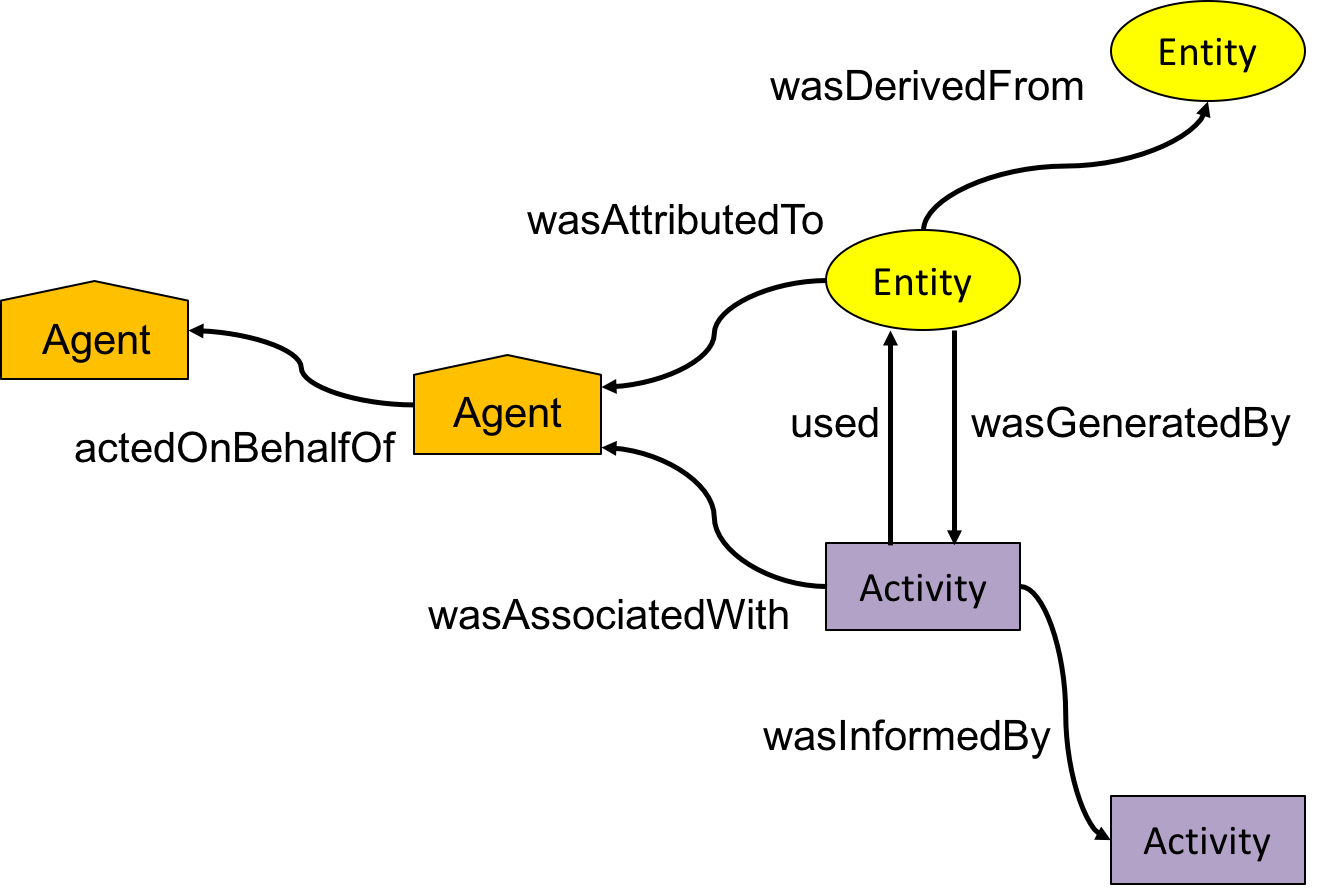
\includegraphics[width=.6\textwidth]{prov_dm_2.PNG}
\end{center}
\caption{Prov-DM respresentation showing types in the model (Entity, Activity, and Agent) and the relationships between them }
\label{prov_rep}
\end{figure}


\par PROV-DM defines the following seven relationships between the types. 

\begin{itemize}
\item wasGeneratedBy: Signifies the production of a new entity by an activity. 

\item used: An entity generated by one activity has been adopted by another activity.

\item wasInformedBy: Signifies the exchange of an entity by two activities.

\item wasDerivedFrom: Represents a copy of information from an entity. 

\item wasAttributedTo: Denotes relational dependency between an entity and an agent when the activity that created the agent is unknown.

\item wasAssociatedWith: An agent created or modified the activity.

\item actedOnBehalfOf: Delegation of authority from an agent to itself or another agent to perform a particular responsibility. 



\end{itemize}


Using the terminology of PROV-DM, we formally define a provenance graph as a labeled directed acyclic graph, $p = (V,E)$ where $V$ is a set of vertices $V =\{v_1,...,v_n\}$ such that $v_i = (type, value)$, with type one of the core types of PROV-DM, and $E$ is a set of edges $E =\{e_1,..., e_n\}$ where $e_i = (v_s, v_d, label)$, with $v_s, v_d$ as source and destination vertices, and $label$ is one of the PROV-DM relations. Two vertices $v_x$, $v_y$ are equal (denoted $ v_x = v_y$) if $v_x.type = v_y.type$ and $v_x.value = v_y.value$. Two edges $e_x $ and $e_y$ are equal (denoted $e_x = e_y$) if $e_x.v_s = e_y.v_s$, $e_x.v_d = e_y.v_d$, and $e_x.label = e_y.label$.  We use the union operator $\cup$ over edge sets in the usual way of the union of sets.



%
%\subsection{Provenance Data Model (Prov-DM)}
%
%Another model for representing provenance data is the Provenance Data Model (PROV\-DM). PROV-DM is a W3C standardized extension of OPM. Prov-DM is a model that is used to depict causal relationships between entities, activities and agents (digital or physical). It creates a common model that allows for interchange of provenance information between heterogeneous devices. It contains two major components: types and relations. 
%
%
%\begin{itemize}
%
%\item Entity: An entity is a physical or digital object. An example of an entity is a file system, a process, or an motor vehicle. An entity may be physical or abstract.
%
%\item Activity: An activity represents some form of action that occurs over a time frame. Actions are acted upon by an agent. An example of an activity is a process opening a file directory, Accessing a remote server.
%
%\item Agent: An agent is a thing that takes ownership of an entity, or performs an activity. An example of an agent is a person, a software product, or a process.
%\end{itemize}
%
%The figure below illustrates the various types contained in PROV-DM and their representation. Entities, activities and agents are represented by oval, rectangle and hexagonal shapes respectively.
%
%\begin{figure}[h]
%\begin{center}
%
%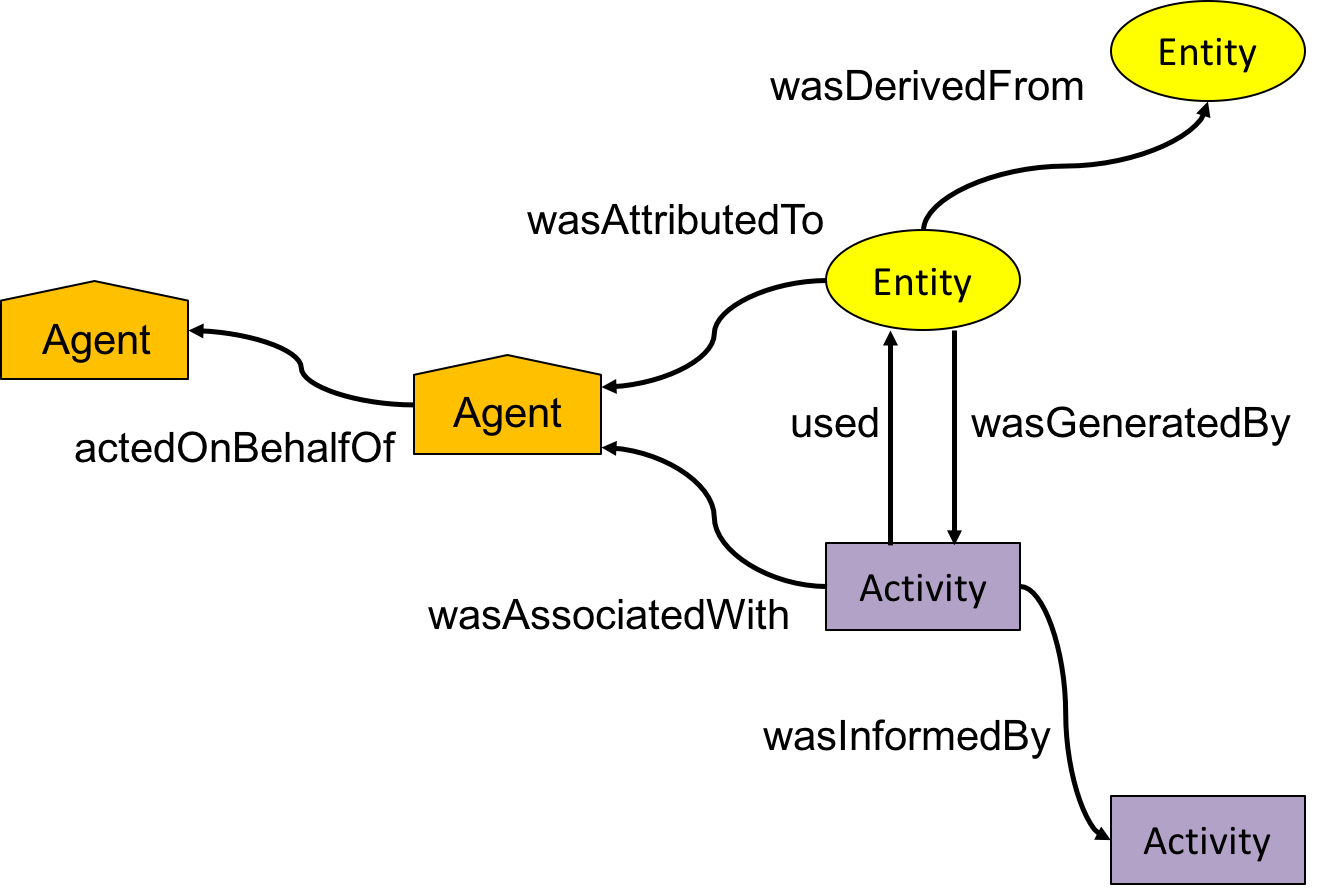
\includegraphics[width=4.0in]{prov_dm_2.PNG}
%\end{center}
%\caption{Prov-DM respresentation showing various types contained in the model (Entity, Activity, and Agent) }
%\end{figure}
%
%Similar to the OPM, PROV-DM does not keep track of future events. PROV-DM relations are outlined below:
%
%
%\begin{itemize}
%\item wasGeneratedBy: This relation signifies the creation of an entity by an activity. 
%
%\item used: This relation denotes that the functionality of an entity has been adopted by an activity.
%
%\item wasInformedBy: This relation denotes a causality that follows the exchange of two activities.
%
%\item wasDerivedFrom: This relation represents a copy of information from an entity. 
%
%\item wasAttributedTo: This denotes relational dependency to an agent. It is used to denote relationship between entity and agent when the activity that created the agent is unknown.
%
%\item wasAssociatedWith: This relation denotes a direct association to an agent for an activity that occurs. This indicates that an agent plays a role in the creation or modification of the activity.
%
%\item actedOnBehalfOf: This relation denotes assigning authority to perform a particular responsibility to an agent. This could be by itself or to another agent.
%
%
%
%\end{itemize}
%
%Some of the difference between OPM and PROV-DM are described below:
%
%\begin{itemize}
%
%\item The main components Artifact, Process and Agent in the OPM model are modified to Entity, Action, and Agent. 
%
%\item Additional causal dependencies such as wasAttributedTo and actedOnBehalfOf were included to represent direct and indirect causal dependencies respectively between agents and entities.
%
%\end{itemize}

%Since PROV-DM is built ontop of OPM and contains easy to understand constructs of types and relations. We are envision are properly represented through the various types and relations, we choose this model to represent provenance data in our IoT architecture instead of OPM. 

%\subsection{PROV-JSON}
%
%PROV-JSON is used for representing PROV-DM data in JSON (JavaScript Object Notation) format. It contains all of the components and relationships contained in PROV-DM and allows for easy serialization and deserialization. JSON is a lightweight data format which is human readable and easy to parse. Figure \ref{provjson} illustrates a use case for the serialization of PROV-DM to PROV-JSON. PROV-JSON contains key-value pairs and can be considered as an indexed version of PROV-DM. The example illustrates the relationship in which s1 tries to access a file (FileB) which was generated by s2. PROV-JSON  contains an entity, activity and agent type which are represented as a json objects and are identified by their respective ids.  Identifiers are optional in PROV-DM but are required for PROV-JSON since json objects contains key-value pairs, the id's of each object has to be implicitly specified and cannot contain null values. 
%
%\begin{figure}[h!]
%\begin{center}
%
%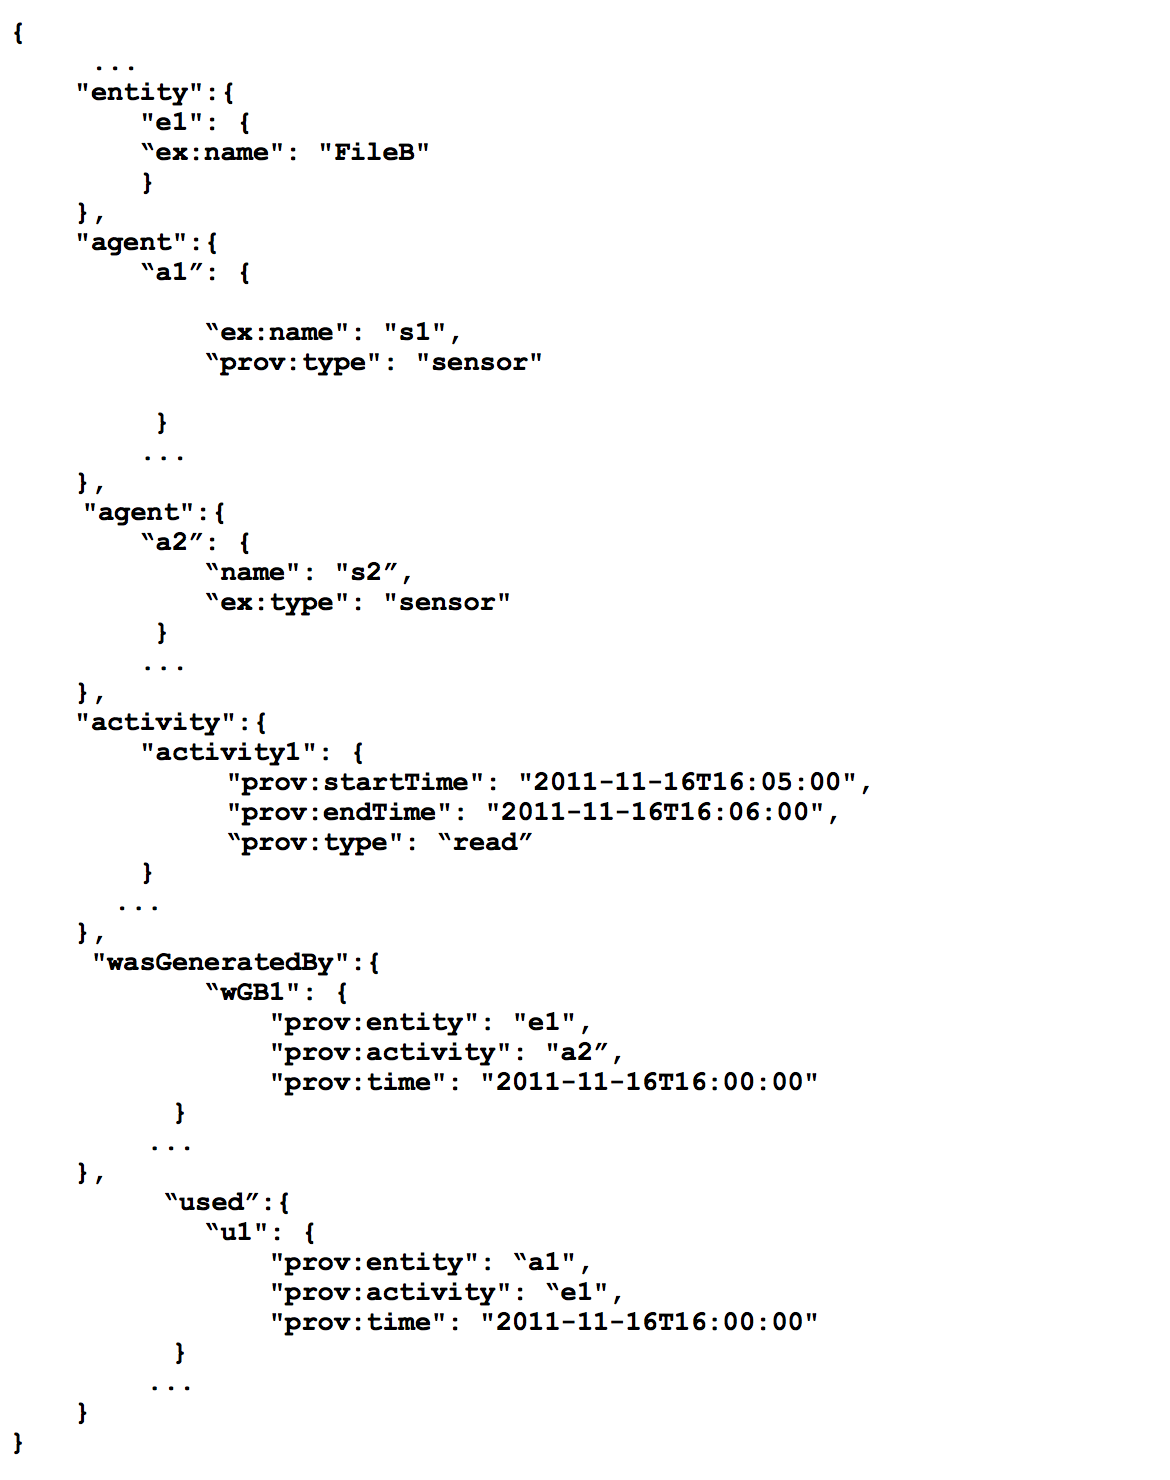
\includegraphics[height=5.7in]{prov_json_edit.png}
%\end{center}
%\caption{PROV-JSON MODEL \copyright \cite{prov_json}}
%
%\label{provjson}
%
%\end{figure}
%
%
%Each object contains fields which assigns additional attributes to the relations (i.e name, type, prov:startTime).  PROV-JSON documents might also contain a prefix object which defines namspaces that are used in the document. In this object is contained a default field which is used to define all of the namespace that contains all other unprefixed namespace.


%\subsection{Similarity Metric} \label{similarity}
%Similarity metric is a measure of how identical two objects are, for example, by measuring the angle between objects (using cosine similarity) or a linear distance (using euclidean distance) between the objects. In this work, we use cosine similarity as our similarity metric. Cosine similarity is a measure of orientation between two non-zero vectors. It measures the cosine of the angle between the vectors. Two vectors which are at an angle of 90\degree  have a similarity of 0, two vectors which are identical (with an angle of 0\degree) have a cosine of 1, and two vectors which are completely opposite (with an angle of 180\degree) have a similarity of -1. Since we are concerned with the similarity of the vectors, we are only concerned with the positive values bounded in [0,1]. To compute the cosine similarity between two vectors, $X$ and $Y$:
%
%\[\mathbf{\cos{(\theta)}} = \dfrac{X \cdot  Y}{ \lVert \mathbf{X} \rVert \cdot \lVert \mathbf{Y} \rVert} =\dfrac{\sum_{i}^n X_i Y_i }{\sqrt[]{\sum_{i}^n X_i^2} \sqrt[]{\sum_{i}^n Y_i^2}}  \]
%
%\subsubsection{Jaccard Similarity}
%This similarity measure evaluates the intersection divided by the union of two non zero vectors.
%
%\[ J(X,Y) = \dfrac{|X \cap Y | }{| X \cup Y |} \]
%
%\subsubsection{Euclidean distance}
%This measures calculates the line distance between two data objects in an euclidean space. The euclidean distance between vectors $X$ and $Y$ , $d(X, Y)$ is defined by: 
%
%\[ d(X, Y) =  \sqrt{\sum_{i=1}^n (X_i - Y_i)^2} \]




%\subsection{A Review of Machine Learning Techniques: $DBSCAN$ and $k$-nearest neighbors}
%
%\subsubsection{$k$-Nearest Neighbors:} $k$-NN is an instance based supervised learning algorithm for data classification. Data is grouped on its similarity to nearest neighbors where $k$ denotes the number of neighbors in which the input data is compared to.  A similarity measure such as euclidean distance, jaccard similarity, or cosine similarity is used to measure the distance between vectors. $k$-NN can be applied to classification and regression problems.
%
%Researchers have proposed various modifications to the $k$-NN algorithm. Ramaswamy et al. \cite{Ramaswamy} proposed a $k$-NN modification which calculates the sparseness estimates for vectors in a dataset. The vectors are sorted in increasing order according the distance from its $k^{th}$ neighbor. Bay and Swabacher demonstrates how pruning irrelevant datapoint which are not considered anomalous can result in a linear complexity of nearest neighbor search for a randomized data. A threshold score is assigned which is based on the score of the weakest anomaly found. Pruning can be achieved by using the  relative density of data points, an anomaly is believed to occur in a group of data points with low density.
%
%\subsubsection{Density Based Spatial Clustering of Applications with Noise ($DBSCAN$):}
%
%\textit{DBSCAN} is a density-based clustering algorithm that differentiates regions with high density from regions with low density. It defines two parameters $\boldsymbol{\varepsilon}$, and $\boldsymbol{MinPts}$. $\varepsilon$ defines the maximum distance between two neighboring points in which they are considered to be in the same cluster. $MinPts$ is the minimum number of points that can be contained in a cluster. 
%
%Let $S = \{s_1, s_2,...s_n \}$ be a set of point to be clustered. $S$ consists of three point categories, a core point, $\boldsymbol{q}$, a border point, $b$ and a noise point, $n$. A core point is a point in which its $minPts$ are within distance $\varepsilon$. These are at the interior of the cluster. Border points are points on the edge of the cluster. A noise point (outlier) is any point that is neither a core point or a border point. A point, $l$ is directly reachable from a core point, $q$ if there exist a path which is within distance of $\varepsilon$ from the core another point. (i.e $ \exists \quad  \{q_1, q_2,...q_n \}, \textrm{where} \quad |q_{i+1}  - q_i| \leq \varepsilon$ ). A core point, $\boldsymbol{q}$ that is within distance $\varepsilon$ (i.e $q \leq \varepsilon$) is considered part of the same cluster. A border point is also considered part of a cluster if it close to a core point. A cluster consists of at least one core point.
%
%
%%\subsubsection{ $k$ means clustering:}



%\subsection{Provenance Graph to Vector Space Conversion }







%\section{Policy Model}
%
%\subsection{eXtensible Access Control Markup Language (XACML)}
% XACML is an access control policy language that allows the creation and enforcement of policies written in XML. It is a standard specification developed by the Organization of Advancement of Structured Information Standards (OASIS). Since it is written in XML, this framework allows for extensible and flexible policy documents. XACML consists of three major components which are involved in policy generation, evaluation and enforcement. The components of XACML are described below: 
% 
% 
% \begin{itemize}
% 
% \item Policy Administration Point (PAP): This component of XACML
%is involved with the generation of policy documents. A Policy document is created by specifications and requirements set aside by an administrator.
%
% \item Policy Decision Point (PDP): The Policy Decision Point evaluates policies by the request context generated by a user. Based on the request, It generates a response (accept,deny or intermediate) This response is communicated with the Policy Enforcement Point which enforces the response sent by the PDP.
%
%
%\item Policy Enforcement Point (PEP):  The Policy Enforcement Point generates request context which is sent to the PDP for evaluation. It is also involved with the responsibility of enforcing request based on decision received by the PDP.
%
% \end{itemize}
% 
% 
% 
% \begin{figure}[tbh]
%\begin{center}
%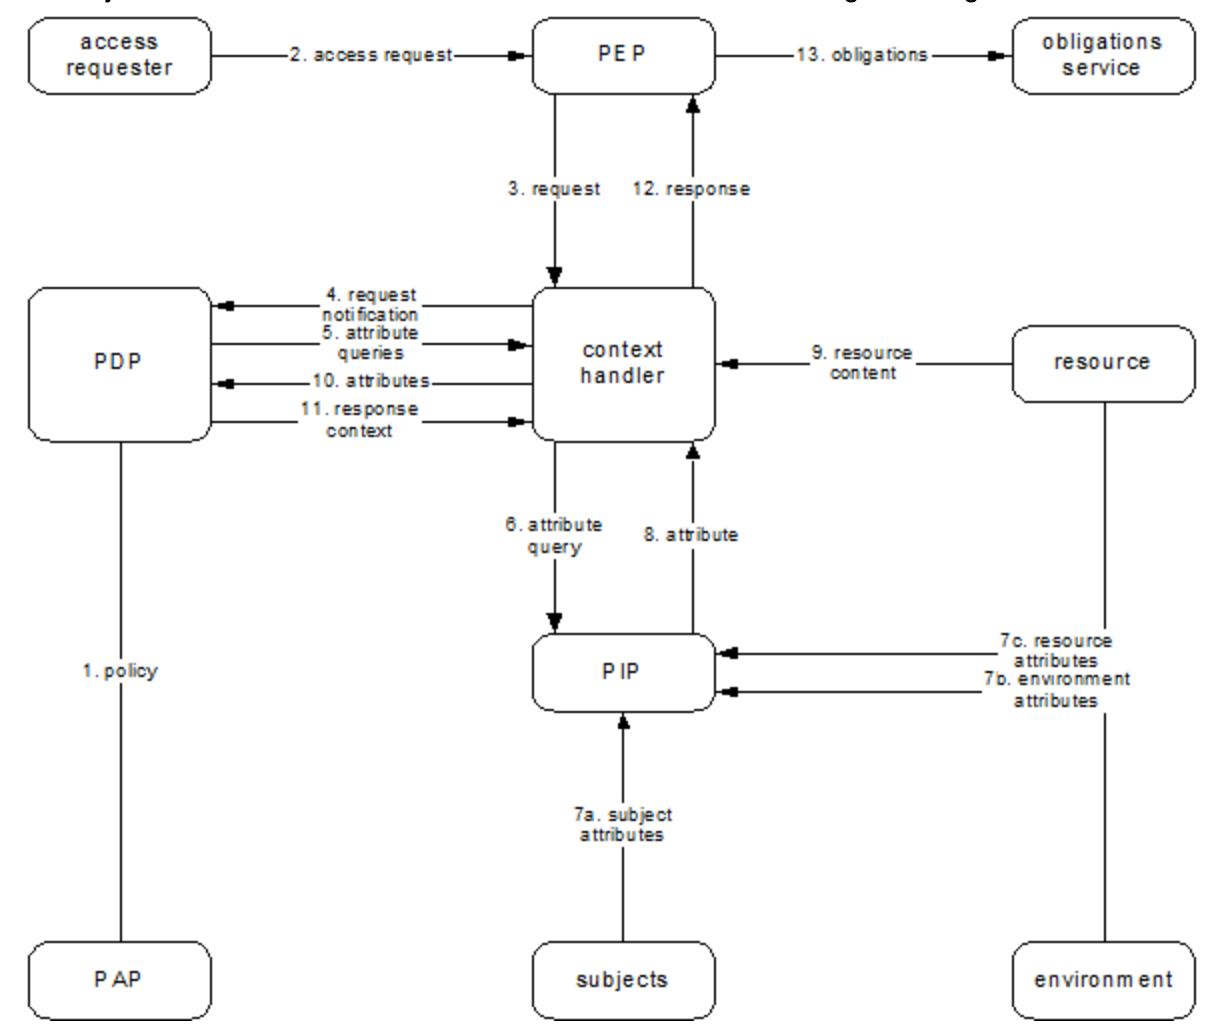
\includegraphics[height=3.5in]{xacml.png}
%\caption{Xacml Data-flow diagram  \copyright \cite{xacml}}
%\end{center}
%\end{figure}
 
%\section{Overview of Relevant Compression techniques}
%
%\subsection{Lossy Compression}
%
%Lossy compression \cite{Sayood:2000:IDC:336428} is a form of data compression in which original data can be reconstructed with some tolerance on loosing some information contained in the original data. This enables higher compression ratio than other compression techniques. Lossy Compression is mostly used in applications that do not contain strict requirements as to loosing some information. An example of a lossless compression application can be seen in an image compression software where the quality of the image is not seen by the naked eye. It is also used in speech transmission. 
%
%\subsection{Lossless Compression}
%Lossless compression \cite{Sayood:2000:IDC:336428} is a data compression technique in which the original data is reconstructed without loss of any information. It can be used by applications which requires that the data is compressed and the original data be identical. An example of such an application that requires lossless compression is text compression.  Any compression that alters the structure of the original text results to a different meaning of the text. For instance, the sentence ``I have a black cat" would have a different meaning if any information is lost from it.
%
%
%
%\subsubsection{Arithmetic Coding}
%
%Arithmetic coding is a form of lossless compression which encodes a stream of characters into a variable size interval between [0,1). A probability is assigned to each characters contained in the string. A cumulative probability is used to calculate the interval of the respective character. Frequent characters are encoded with shorter codes than less frequent characters. 


%\subsection{Anomaly Detection}
%
%The notion of what constitutes an anomaly is often domain specific. Hawkins defines an anomaly as an ``observation which deviates so much from the other observations as to arouse that it was generated by a different mechanism" \cite{hawkins}. In computing, an anomaly often indicates the presence of a malicious intrusion or a system fault. For example, an anomaly could be a sudden increase in web traffic of a web server which could be indicative of a denial of service attack. Additionally, in a critical care health device such as a pacemaker, an anomalous event could be detrimental to the health of a patient which could result in the loss of life. 
%
%Anomaly detection consists of two phase, learning phase also known as the training phase and the test also known as the detection phase. In the training phase, the system collects training dataset. This data is considered to be a representation of the system's normal daily activity and free from malicious events. Once training dataset has been collected, the system's activities are further observed. This part is known as the testing phase. In the testing phase,  observed system behavior is compared to the learning phase to determine is an anomaly exists between the two. A threshold as defined by domain experts is used to determine if the observed data is considered an anomaly.
%
%Data labels are grouped into three major categories. Supervised anomaly detection, semi-supervised anomaly detection, and unsupervised anomaly detection. In supervised anomaly detection approach, training data contains instances of normal and anomalous data. Incoming data is classified based on the training data category. In semi-supervised approach, only one class of training data is collected, normal data. Incoming data that does not fit the normal class as specified by a threshold is regarded as an anomalous. In the training phase, most anomaly detection techniques use data derived from the normal system behavior.  This is referred to as one class classification. In unsupervised approach, there are no training dataset. it is believed that normal data is clustered around each and occurs more frequently than an anomaly. This is a widely used form of anomaly detection since training data which is hard to get is not requited. 
%
%
%Anomaly detection involves the use of rule-based, statistical, clustering or classification techniques to determine normal or anomalous data instances. The process of determining all anomalous instances in a given dataset or system is a complex task. A major challenge in anomaly detection is providing the right feature set from the data to use for detection. Another challenge exists in defining what constitutes as normal system behavior. Most anomaly detection using point based data often fail to include the dependencies that exist between data points. 




%Graphs offers a means of modeling complex structures such as social networks, computer networks, biological DNA sequences.  




%Details on anomaly detection techniques are outlined below
%
%
%\begin{enumerate}[]
%
%
%\item Statistical-based approach: This approach involves the use of parametric or non parametric statistical inference to develop models which are used to determine if a dataset fits a statistical model. Instances that do not fit the defined statistical model are classified as an anomaly. 
%
%\item Classification: The main idea in this approach involves building models which use training data set with predefined labels (i.e normal, anomalous) to classify incoming data. Classification works in two phase: training phase and observation phase. In the training phase, data is collected which contains labels of normal and anomalous system behavior. If the dataset only contains a label of either anomalous or normal behavior, this is considered as a one class classifier. In the observation phase, incoming data is classified by defined data labels.
%\begin{itemize}
%
%\item Nearest-Neighbor: It is based on the assumption that normal data occurs in dense neighborhoods and abnormal data in sparse neighborhoods. The main idea is to assign an incoming observation data to a class based on its proximity to the closest data point in the training data set. A distance or similarity measure is used to quantify the distance between points in a dataset.  A popular form of nearest neighbor technique is the $k$-nearest neighbor which groups incoming data based on proximity to $k$ closest data point. Details on $k$- nearest neighbors is discussed in section 3.5. 
%
%\end{itemize}
%
%\item Clustering: The main idea is to group similar data instances into clusters. There are various approach to clustering. One approach looks at the density of the clusters, normal data belongs to large dense clusters while abnormal data belongs to small clusters. Another approach as treats clustering as one class which assumes that normal belongs to a cluster and abnormal data does not. Another approach looks at the distance of the data to the centroid. Centroids are seen as the center of the cluster. Normal data are  considered to be closer to the centroid than anomalies lie.
%
%\begin{itemize}
%
%\item Density: This approach is used to estimate the density of  $k$ nearest neighbors. A data instance in a dense neighborhood is considered normal while data instances in neighborhoods with a sparse density are considered anomalous. The distance from a data instance to a nearest neighbor is seen as the inverse of the density of data instances.  This approach faces an issue in which the density approach performs poorly in regions of varying densities. Local outlier factor addresses this issue. Local outlier factor is a measure of the degree of Outlieriness of each data instance contained in a data set. It is achieved by comparing the ratio of local density of k nearest neighbors to the density of a data instance. Data instances with lower density are considered outliers.
%
%\end{itemize}
%
%
%
%
%
%
%\end{enumerate}  



